\documentclass[a4j, titlepage]{jarticle}

%% プリアンブル部 %%
\usepackage[table]{xcolor}
\usepackage{xurl}
\usepackage{ascmac}
\usepackage[dvipdfmx]{graphicx}
\usepackage{listings}
\usepackage{comment}
\usepackage{fancybox,ascmac}
\usepackage[most]{tcolorbox}

\title{情報工学実験II\\ソーティングプログラム}
\author{ライモン ウィジャヤ}
\date{2021-05-21}
\begin{document}

\maketitle
\tableofcontents
\clearpage

\section{概要}
少量または大量なデータに対して, 小さい順(昇順)または大きい順(降順)に並び替えする作業はソーティングである.データをソーティング時間が早ければ早いほどソーティングの効率がいいと言える. ソーティングの中ではたった一つのソーティング方法でどんな数値列を早くソーティングするのはない. 次はソーティングアルゴリズムをいくつか紹介する. どんなアルゴリズムを持ってるか, どれぐらいデータをソーティングする時間がかかるかなどを説明する. 

アルゴリズムに従って計算を実行をそのアルゴリズムの\textbf{時間計算量}(\textit{time complexity})と呼び, 例えば, あるnデータに対してそのアルゴリズム計算量を表し方はオーダー(\textit{O}(n))と記す.

全プログラムのコードはC言語で書いている. 用意乱数データは七つあり, それぞれの特徴は ~表\ref{table:data-type}に載せている. 
\begin{table}[bth]
\label{table:data-type}
\caption{データタイプ}
\begin{center}
\begin{tabular}{lc}
\hline
データ & タイプ \\ \hline\hline
data 1-3 & 乱数 \\
data 4  & 昇順 \\ 
data 5 & 降順 \\
data 6 & バイトニック \\
data 7 & ジグザグ \\ \hline
\end{tabular}
\end{center}
\end{table}

%%-------------%%
%% BUCKET SORT %%
%%-------------%%
\section{バケットソート}
バケットソートとは、別名バケツソートとも呼ばれ, あらかじめ順番通り並べて準備されたバケツに, データを放り込むことで並べ替えを行おうという, いささか乱暴なソートアルゴリズムである.

\begin{figure}[tbh]
\centering \includegraphics[height=5.4cm, keepaspectratio]{bukcet.png}
\caption{バケットソートイメージ}
\label{bucket}
\end{figure}

この方法は, データの存在する範囲が有限個に限定されていないと使えませんが, 使える場合は非常に高速に並べ替えを実行できる, きわめて有用なアルゴリズムである. イメージは図\ref{bucket}のようにである.

\subsection{プログラム}
以下はバケットソートのプログラムである.\vspace{5pt}
\lstset{backgroundcolor=\color{green!20!}, frameround=fttt}
\begin{lstlisting}[basicstyle=\ttfamily\footnotesize, frame=trbl]
#include<stdio.h>
#include<stdlib.h>
#include<time.h>
#define N 100000

int maxval(int a[])
{
    int max = a[0];
    int i;
  
    for(i = 1; i < N; i++){
        if(max < a[i]){
            max = a[i];
        }
    } 
    return max;
}

void bucket_sort(int number[], int maxvalue)
{
    int bucket[maxvalue + 1];
    int i,j, counter;

    for(i = 0; i <= maxvalue; i++){
        bucket[i] = 0;
    }

    for(i = 0; i < N; i++){
        bucket[number[i]] += 1;
    }
    
    j = 0;
    for(i = 0; i <= maxvalue; i++){
        if (bucket[i] != 0){
            counter = bucket[i];
            while(counter > 0){
                number[j] = i;
                j++; counter--;
            }
        }
    }
}

int main(int argc, char *argv[]){
    FILE *fp1; FILE *fp2;
    int number[N];
    int i;
    int maxvalue;
    
/*------- ファイルからデータの読み込み ---------*/
    if(argc != 2){                         
        puts("Parameter Error");
        return 0;
    }
    if ((fp1 = fopen(argv[1], "r")) == NULL){
        puts("NO FILE WITH THAT NAME");
        return 0;
    }
    for(i = 0; i < N; i++){
        fscanf(fp1, "%d", &number[i]);
    }
    fclose(fp1);
    
/*------- プログラム処理 ---------*/
    clock_t begin = clock();
    maxvalue = maxval(number);
    bucket_sort(number, maxvalue);
    clock_t end = clock();

    fp2 = fopen("./output000.dat", "w");
    for(i = 0; i < N; i++){
        fprintf(fp2, "%d\n", number[i]);
    }
    fclose(fp2);
    puts("Done!");
    printf("The elapsed time is %lf sec\n", (double)(end-begin)/CLOCKS_PER_SEC);
    return 0;
}
\end{lstlisting}

\subsection{動作}
まずは数値データを読み込んで, 数値データの中でmaxval()関数で最大値を探索する. 最大値とデータの配列をbucket\_sort()関数に渡す.

bucket\_sort()関数の中に次の動作が行われている.
\begin{enumerate}
\item バケットを最大値$+1$用意して, 値を初期化する. 
\item 数値データと配列のインデックスが依存するので, 読み込んだ数値が配列のその数値のバケット(インデックス)を1増やす. 
\item 全数値を読み込んだ後は, 元配列に一つずつバケットの中身を順番で書き込む.
\item ソート完了.
\end{enumerate}

\subsection{時間計算量}
まずはバケットをm個を準備する時間計算量は\textit{O}(m)である. 次はn数値データをバケットに入れる時間計算量は\textit{O}(n)である. バケットソートの計算量は\textit{O}(m + n)である. 次は最大値を求める時間計算量は\textit{O}(n)なので, このプログラム全体時間計算量は\textit{O}(m + 2n)である. 

以下の表\ref{table:bucket}は上のコードで実行したソート計算時間だ.(CPUはintel i7 $7^{th}$ Gen, RAMは8GB)
\begin{table}[bth]
\label{table:bucket}
\caption{計算時間(バケットソート)}
\begin{center}
\begin{tabular}{|l|ccccccc|}
\hline
データ & data1 & data2 &data3 &data4 &data5 &data6 &data7 \\ \hline
計算時間(秒) & 0.001324 & \cellcolor{green!20}0.001296 & 0.001612 & \cellcolor{red!20} 0.001891 & 0.001387 & 0.001546 & 0.001351\\ \hline
\end{tabular}
\end{center}
\end{table}

表\ref{table:bucket}より, 数値データ間の計算時間の差はあまり多くないから, 数値データが乱数や降順や昇順など関係ない.  


%%-------------%%
%% INSERT SORT %%
%%-------------%%
\section{挿入ソート}
挿入ソートは比較によりソーティングを行うアルゴリズムである. 図\ref{insert}を見たらわかりやすい. 
\begin{figure}[tbh]
\centering 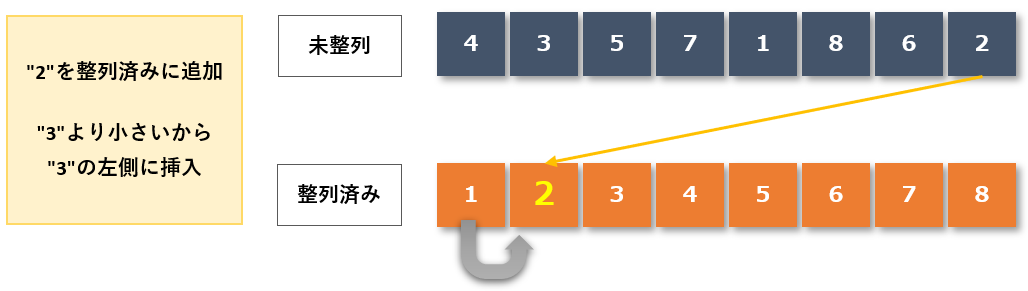
\includegraphics[height=4cm, keepaspectratio]{insertionSort.png}
\caption{挿入ソートイメージ}
\label{insert}
\end{figure}
具体的に言うと, 整列してある配列に追加要素を適切な場所に挿入するアルゴリズムである.

\subsection{プログラム}
以下はバケットソートのプログラムである.\vspace{5pt}
\lstset{backgroundcolor=\color{green!20!}, frameround=fttt}
\begin{lstlisting}[basicstyle=\ttfamily\footnotesize, frame=trbl]
%% ENTER THE PROGRAM %%
#include<stdio.h>
#include<stdlib.h>
#include<time.h>
#define N 100000

void swap(int *a, int *b){
    int tmp;
    tmp = *a;
    *a = *b;
    *b = tmp;
}

void insertion(int number[])
{
    int i, j, tmp;

    for(i=1; i < N; i++){
        tmp = number[i];
        j = i;
        while((j > 0) && (number[j-1] > tmp)){
            number[j] = number[j-1];
            j--;
        }
        number[j] = tmp;   
    }
}


int main(int argc, char *argv[])
{
    FILE *fp1;
    FILE *fp2;
    int number[N];
    int i = 0;

    if(argc != 2){                         
        puts("Parameter Error");
        return 0;
    }

    if ((fp1 = fopen(argv[1], "r")) == NULL){
        puts("NO FILE WITH THAT NAME");
        return 0;
    }

    for(i = 0; i < N; i++){
        fscanf(fp1, "%d", &number[i]);
    }

    fclose(fp1);
/*------- プログラム処理 ---------*/
    clock_t begin = clock();
    insertion(number);
    clock_t end = clock();

    fp2 = fopen("./output000.dat", "w");
    for(i = 0; i < N; i++){
        fprintf(fp2, "%d\n", number[i]);
    }
    fclose(fp2);

    puts("Done!");
    printf("The elapsed time is %lf sec\n", (double)(end-begin)/CLOCKS_PER_SEC);

    return 0;
}
\end{lstlisting}
\subsection{動作}
まずはi, j, tmp(一時的なものという)変換を用意する. 次はソート動作に入る.
\begin{enumerate}
\item tmp変数に配列number[i]を入れ, j変数はi変数の値を持たせる. j変数は前に何個数値データがどれぐらいあるかを表すものだ. 
\item tmp変数の値より大きかったら, それらの値いを入れ替える [$number[j] = number[j-1]$]ともにjの値が1減る.
\item tmp変換の値がnumber[$j-1$]より高かったらループが終わりで, 最後にnumber[j]にtmpの値を入れる(その値の適切な場所である).  
\item これはiがNまで繰り返す
\item ソートは終わり
\end{enumerate}

\subsection{時間計算量}
格時点で着目している$a_i$を, その時までにソートされている系列($a_1$, $a_2$, \dots, $a_{i-1}$)の間の適切な場所に挿入するというもので, $a_i$より大きい数値を右シフトするので時間計算量\textit{O}($n^2$)である.

以下の表\ref{table:insert}は上のコードで実行したソート計算時間だ.(CPUはintel i7 $7^{th}$ Gen, RAMは8GB)
\begin{table}[bth]
\label{table:insert}
\caption{計算時間(挿入ソート)}
\begin{center}
\begin{tabular}{|l|ccccccc|}
\hline
データ & data1 & data2 &data3 &data4 &data5 &data6 &data7 \\ \hline
計算時間(秒) & 5.858170 & 5.826343 & 5.757950 & \cellcolor{green!20}0.000317 & \cellcolor{red!20} 11.601440 & 5.764131 & 5.863555\\ \hline
\end{tabular}
\end{center}
\end{table}
data4は昇順データなのでソート処理は全くないから, 一瞬で終わる. しかし, 降順データdata5に対して, これは最悪状況から,
一番遅かった.このソート方はランダムのデータに対して, 少し有効だ.





%%-------------%%
%% BUBBLE SORT %%
%%-------------%%
\section{バブルソート}
バブルソートは配列において隣り合うふたつの要素の値を比較して条件に応じた交換を行う整列アルゴリズムです. 条件とは値の大小関係です.「値の大きい順(降順)」か「値の小さい順(昇順)」に配列を並び替えます. 図\ref{bubble}がバブルソートのイメージだ.
\begin{figure}[tbh]
\centering \includegraphics[height=4cm, keepaspectratio]{bubble.png}
\caption{バブルソートイメージ}
\label{bubble}
\end{figure}

\subsection{プログラム}
以下はバケットソートのプログラムである.\vspace{5pt}
\lstset{backgroundcolor=\color{green!20!}, frameround=fttt}
\begin{lstlisting}[basicstyle=\ttfamily\footnotesize, frame=trbl]
%% ENTER THE PROGRAM %%
#include<stdio.h>
#include<stdlib.h>
#include<time.h>
#define N 100000

void swap(int *a, int *b){
    int tmp = *a;
    *a = *b;
    *b = tmp;
}

void bubble_sort(int number[]){
    int i,j, sorted;
    j = N;
    do{
        sorted = 1; j=j-1;
        for(i=1; i <= j; i++){
            if(number[i-1] > number[i]){
                swap(&number[i-1], &number[i]);
                sorted = 0;
            }
        }
    } while(!sorted);
}


int main(int argc, char *argv[])
{
    FILE *fp1;
    FILE *fp2;
    int number[N];
    int i;

    if(argc != 2){                         
        puts("Parameter Error");
        return 0;
    }

    if ((fp1 = fopen(argv[1], "r")) == NULL){
        puts("NO FILE WITH THAT NAME");
        return 0;
    }

    for(i = 0; i < N; i++){
        fscanf(fp1, "%d", &number[i]);
    }

    fclose(fp1);
/*------- プログラム処理 ---------*/
    clock_t begin = clock();
    bubble_sort(number);
    clock_t end = clock();

    fp2 = fopen("./output000.dat", "w");
    for(i = 0; i < N; i++){
        fprintf(fp2, "%d\n", number[i]);
    }
    fclose(fp2);

    puts("Done!");
    printf("The elapsed time is %lf sec\n", (double)(end-begin)/CLOCKS_PER_SEC);
    return 0;
}
\end{lstlisting}
\subsection{動作}
バブルソートのアルゴリズムは以下通り行われている.
\begin{enumerate}
\item 先頭の要素'A'と隣り合う次の要素'B'の値を比較する
\item 要素'A'が要素'B'より大きいなら、要素'A'と要素'B'の値を交換する
\item 先頭の要素を'B'に移し、要素'B'と隣り合う要素'C'の値を比較/交換する
\item 先頭の要素を'C','D','E'...と移動しながら比較/交換をリストの終端まで繰り返す
\item 最も大きい値を持つ要素が配列の終端へ浮かびあがる
\item 配列の終端には最も大きな値が入っているので、配列の終端の位置をずらして(j変数をひとつ減らして)手順1〜6を繰り返す
\end{enumerate}

\subsection{時間計算量}
配列がn個データを持つとすると, 一番目の要素が$n-1$回スキャンし, 2番目の要素が$-2$回スキャンし, $n-1$番目の要素までだから, $n-1 + n-2 + \dots + 1$で, 
結果は$\frac{n}{2}\times(n)$ということだ.つまりバブルソートの時間計算量は\textit{O}($n^2$)である.

以下の表\ref{table:bubble}は上のコードで実行したソート計算時間だ.(CPUはintel i7 $7^{th}$ Gen, RAMは8GB)
\begin{table}[bth]
\label{table:bubble}
\caption{計算時間(バブルソート)}
\begin{center}
\begin{tabular}{|l|ccccccc|}
\hline
データ & data1 & data2 &data3 &data4 &data5 &data6 &data7 \\ \hline
計算時間(秒) & 31.203036 & \cellcolor{red!20}31.283206 & 31.235534 & \cellcolor{green!20}0.000248 &  22.961952 & 16.764867 & 27.256440\\ \hline
\end{tabular}
\end{center}
\end{table}
表\ref{table:bubble}を見ると, 乱数のデータが一番時間がかかるということがわかる. バイトニックやジグザグデータは昇順データ以外よりやや早いということがわかる.

%%-------------%%
%% SHAKER SORT %%
%%-------------%%
\section{シェーカーソート}
バブルソートを、効率がよくなるように改良したものだ. 別名は、双方向バブルソート, 改良交換法である.

バブルソートではスキャンを一方向にしか行わないのに対し, シェーカーソートでは交互に二方向に行う. バブルソートと同じく安定な内部ソートである. 図\ref{shaker}はシェーカーソートのイメージだ.

\begin{figure}[tbh]
\centering \includegraphics[height=5cm, keepaspectratio]{shaker.jpg}
\caption{シェーカーソートイメージ}
\label{shaker}
\end{figure}

\subsection{プログラム}
以下はバケットソートのプログラムである.\vspace{5pt}
\lstset{backgroundcolor=\color{green!20!}, frameround=fttt}
\begin{lstlisting}[basicstyle=\ttfamily\footnotesize, frame=trbl]
#include<stdio.h>
#include<stdlib.h>
#include<time.h>
#define N 100000

void swap(int *a, int *b){
    int tmp = *a;
    *a = *b;
    *b = tmp;
}

void shaker_sort(int number[]){
    int i, j;
    int right, left;
    int sorted = 0;

    left = 0;
    right = N - 1;

    while (left != right){
        for(i = left; i < right; i++){
            if(number[i] > number[i + 1]){
                swap(&number[i], &number[i + 1]);
                sorted = i;
            }
        }
        right = sorted;

        for(i=right; i > left; i--){
            if(number[i] < number[i-1]){
                swap(&number[i-1], &number[i]);
                sorted = i;
            }
        }
        left = sorted;
    }    
}



int main(int argc, char *argv[])
{
    FILE *fp1;
    FILE *fp2;
    int number[N];
    int i = 0;

    if(argc != 2){                         
        puts("Parameter Error");
        return 0;
    }

    if ((fp1 = fopen(argv[1], "r")) == NULL){
        puts("NO FILE WITH THAT NAME");
        return 0;
    }

    for(i = 0; i < N; i++){
        fscanf(fp1, "%d", &number[i]);
    }

    fclose(fp1);
/*------- プログラム処理 ---------*/
    clock_t begin = clock();
    shaker_sort(number);
    clock_t end = clock();

    fp2 = fopen("./output000.dat", "w");
    for(i = 0; i < N; i++){
        fprintf(fp2, "%d\n", number[i]);
    }
    fclose(fp2);

    puts("Done!");
    printf("The elapsed time is %lf sec\n", (double)(end-begin)/CLOCKS_PER_SEC);
    return 0;
}

\end{lstlisting}
\subsection{動作}
シェーカーソートの動作は以下通りである.
\begin{enumerate}
\item right, left変数を用意し, rightにN-1でleftに0を入れる
\item 左から始まり, A要素と隣り合う次のB要素と比較し, もしBがAより小さかったらスワップし, rightのところまでこの動作をする. 
\item 終わったら, 右側に何番までスワップするか新しい値がright変数に入れる.
\item 動作の2番と同じ動作が行うが, 逆で右から始まり, 終わったら, 左側に何番までスワップするか新しい値がleft変数に入れる.
\item 動作2番目から4番目までを繰り返し, right変数とleft変数の値が同じになったら, ソートが終わり. 
\end{enumerate}

\subsection{時間計算量}
シェーカーソートはバブルソートのと同じく最悪状況で時間計算量は\textit{O}($n^2$)である. ただバブルソートの無駄な部分を少し省いたから, バブルソートより早いということになる.

以下の表\ref{table:shaker}は上のコードで実行したソート計算時間だ (CPUはintel i7 $7^{th}$ Gen, RAMは8GB). 
表\ref{table:shaker}を見ると, バブルソートの計算時間より少し早かったということがわかる.降順データに対するソーティングは一番時間がかかるが, データ1-3番目まではデータ5とあまり違わない.
\begin{table}[bth]
\label{table:shaker}
\caption{計算時間(シェーカーソート)}
\begin{center}
\begin{tabular}{|l|ccccccc|}
\hline
データ & data1 & data2 &data3 &data4 &data5 &data6 &data7 \\ \hline
計算時間(秒) & 23.967871 & 24.600001 & 24.405949 & \cellcolor{green!20}0.000630 &  \cellcolor{red!20}25.807042 & 14.228346 & 20.016187\\ \hline
\end{tabular}
\end{center}
\end{table} 
\pagebreak

%%-------------%%
%%  QUICK SORT %%
%%-------------%%
\section{クイックソート}
データの比較と交換回数が非常に少ないのが特徴で, 一般的なばらばらデータ(ランダムに散らばっているデータ)に対して, 最も効率良く並べ替えを実行します. クイックソートのイメージは図\ref{quick}である. 
クイックソートは, 実用上もっとも高速であるとされている並べ替えアルゴリズムで, 多くのプログラムで利用されている.

\begin{figure}[tbh]
\centering \includegraphics[height=5cm, keepaspectratio]{quick.jpeg}
\caption{クイックソートイメージ}
\label{quick}
\end{figure}

\subsection{プログラム}
以下はバケットソートのプログラムである.\vspace{5pt}
\lstset{backgroundcolor=\color{green!20!}, frameround=fttt}
\begin{lstlisting}[basicstyle=\ttfamily\footnotesize, frame=trbl]
#include<stdio.h>
#include<stdlib.h>
#include<time.h>
#define N 100000

void swap(int* a, int* b)
{
    int t = *a;
    *a = *b;
    *b = t;
}

int partition(int arr[], int low, int high)
{
    int pivot = arr[high];
    int i = (low - 1); 
    for (int j = low; j <= high - 1; j++)
    {
        if (arr[j] < pivot)
        {
            i++; 
            swap(&arr[i], &arr[j]);
        }
    }
    swap(&arr[i + 1], &arr[high]);
    return (i + 1);
}

void quick_sort(int arr[], int low, int high)
{
    if (low < high)
    {
        int pi = partition(arr, low, high)
        
        quick_sort(arr, low, pi - 1);
        quick_sort(arr, pi + 1, high);
    }
}


int main(int argc, char *argv[])
{
    FILE *fp1;
    FILE *fp2;
    int number[N];
    int i = 0;

    if(argc != 2){                         
        puts("Parameter Error");
        return 0;
    }

    if ((fp1 = fopen(argv[1], "r")) == NULL){
        puts("NO FILE WITH THAT NAME");
        return 0;
    }

    for(i = 0; i < N; i++){
        fscanf(fp1, "%d", &number[i]);
    }

    fclose(fp1);
/*------- プログラム処理 ---------*/
    clock_t begin = clock();
    quick_sort(number, 0, N-1);
    clock_t end = clock();

    fp2 = fopen("./output000.dat", "w");
    for(i = 0; i < N; i++){
        fprintf(fp2, "%d\n", number[i]);
    }
    fclose(fp2);

    puts("Done!");
    printf("The elapsed time is %lf sec\n", (double)(end-begin)/CLOCKS_PER_SEC);
    return 0;
}
\end{lstlisting}
\subsection{動作}
クイックソートの動作は以下通り行われている.
\begin{enumerate}
\item partition関数がpivotのインデックスを返して, partition関数の中に, pivotの値が決められ, pivotの値より小さかったら左にインデックスiとスワップし, iを1増やす. 
\item 1番目の動作はhigh変数の値まで繰り返す. 最後にpivotのインデックスと値がインデックスiのところに入れる. 
\item  pivotに区切られたデータが動作1-2が行って, 繰り返し, ソート完了.
\end{enumerate}
\subsection{時間計算量}
最悪の場合は分割が1と$N-1$に行われつづけた場合で、この場合、クイックソートの分割の深さはNとなり, それぞれのデータの深さはN, N, $N-1$, $N-2$, \dots, 3, 2となる. したがって, この場合のクイックソートの計算時間は, 
\begin{equation}
N + N + N-1 + N-2 + \dots + 3 + 2 = \frac{N^2}{2} + \frac{3N}{2} - 1
\end{equation}

となり, 時間計算量は\textit{O}($N^2$)となる.

また, 平均的な場合として, すべて異なる一様分布のデータに対しては, \textit{O}(N $\log N$) になることが知られている.

以下の表\ref{table:quick}は上のコードで実行したソート計算時間だ (CPUはintel i7 $7^{th}$ Gen, RAMは8GB). 
表\ref{table:quick}を見ると, 乱数データに対しては, 計算時間一番早いということがわかる. 昇順データと降順データが最悪の場合でるから, 一番遅いということがわかる.
\begin{table}[bth]
\label{table:quick}
\caption{計算時間(クイックソート)}
\begin{center}
\begin{tabular}{|l|ccccccc|}
\hline
データ & data1 & data2 &data3 &data4 &data5 &data6 &data7 \\ \hline
計算時間(秒) & 0.023820 & \cellcolor{green!20}0.016687 & 0.025379 & \cellcolor{red!20}10.638173 & 10.125896 & 2.043179 & 0.014155\\ \hline
\end{tabular}
\end{center}
\end{table} 
\pagebreak

\section{ソートアルゴリズムの比較}
表\ref{table:hikaku}はソートアルゴリズムの計算時間を比べる表である.

\begin{table}[bth]
\label{table:hikaku}
\caption{計算時間の比較}
\begin{center}
\begin{tabular}{|l|c|c|c|c|c|}
\hline
      & バケツソート & 挿入ソート & バブルソート & シェーカーソート & クイックソート \\\hline
data1 & 0.001324 &  5.858170 & 31.203036 & 23.967871 &  0.023820 \\ \hline
data2 & \cellcolor{green!20}0.001296 &  5.826343 & \cellcolor{red!20}31.283206 & 24.600001 &  \cellcolor{green!20}0.016687 \\ \hline
data3 & 0.001612 &  5.757950 & 31.235534 & 24.405949 &  0.025379 \\ \hline
data4 & \cellcolor{red!20}0.001891 &  \cellcolor{green!20}0.000317 &  \cellcolor{green!20}0.000248 &  \cellcolor{green!20}0.000630 & \cellcolor{red!20}10.638173 \\ \hline
data5 & 0.001387 & \cellcolor{red!20}11.601440 & 22.961952 & \cellcolor{red!20}25.807042 & 10.125896 \\ \hline
data6 & 0.001546 &  5.764131 & 16.764867 & 14.228346 &  2.043179 \\ \hline
data7 & 0.001351 &  5.863555 & 27.256440 & 20.016187 &  0.014155 \\ \hline
\end{tabular}
\end{center}
\end{table} 

表\ref{table:hikaku}を見ると, こんな事をまとめることができる
\begin{enumerate}
\item バケットソートはどんなソートアルゴリズムより早いということがわかる. だが,無駄なメモリが非常に使ってしまう.
\item data1に対して, クイックソートやバケットソートが早くソートされる.
\item 昇順並びなので, data5に対して, クイックソートや挿入ソートが早くソートされる.
\item バブルソートとシェーカーソートは比較回数が多いため, 計算が遅いということがわかる. 同じ計算時間量\textit{O}($n^2$)で挿入ソートが一番早い.
\end{enumerate}
\pagebreak
\section{他のソートアルゴリズム(ツリーソート)}
ツリーソートはソーティングをするのに, 二分木が作られ, 次に、要素がソートされた順序で出てくるように, ツリーを(順番に)トラバースするアルゴリズムである. 図\ref{tree}ではソートの動作が描いてある. 

\begin{figure}[tbh]
\centering \includegraphics[height=10cm, keepaspectratio]{treesort.jpg}
\caption{ツリーソートのイメージ}
\label{tree}
\end{figure}

\subsection{時間計算量}
平均的なケースでは, 二分木にnノードを挿入する時間の複雑さは\textit{O}(n$\log n$) のオーダーだ.これは, 形成される二分木がバランスのとれた二分木である場合に発生する. したがって, 時間の複雑さは\textit{O}(n$\log n$)である.

最悪の場合は, 配列がソートされ、最大高さ\textit{O}(n)の不均衡な2値探索木が形成される. 高さが$\log n$の通常の二分木の場合の探索時間は\textit{O}($\log n$)であるのに対し, 探索には\textit{O}(n)時間, 挿入には\textit{O}($n^2$)が必要. 最悪の場合の時間的複雑さは\textit{O}($n^2$)である.

ベストケースは形成された二値探索木が均衡している場合である. 最良の時間複雑度は\textit{O}(n$\log n$). これは平均ケースの時間複雑度と同じ.
\end{document}